\documentclass[11pt]{article}
\usepackage[margin=1in,paperwidth=9in,paperheight=7in]{geometry}
\usepackage{graphicx}
\usepackage{caption}
\pagestyle{empty}
\setlength{\parindent}{0pt}

\begin{document}

\begin{center}
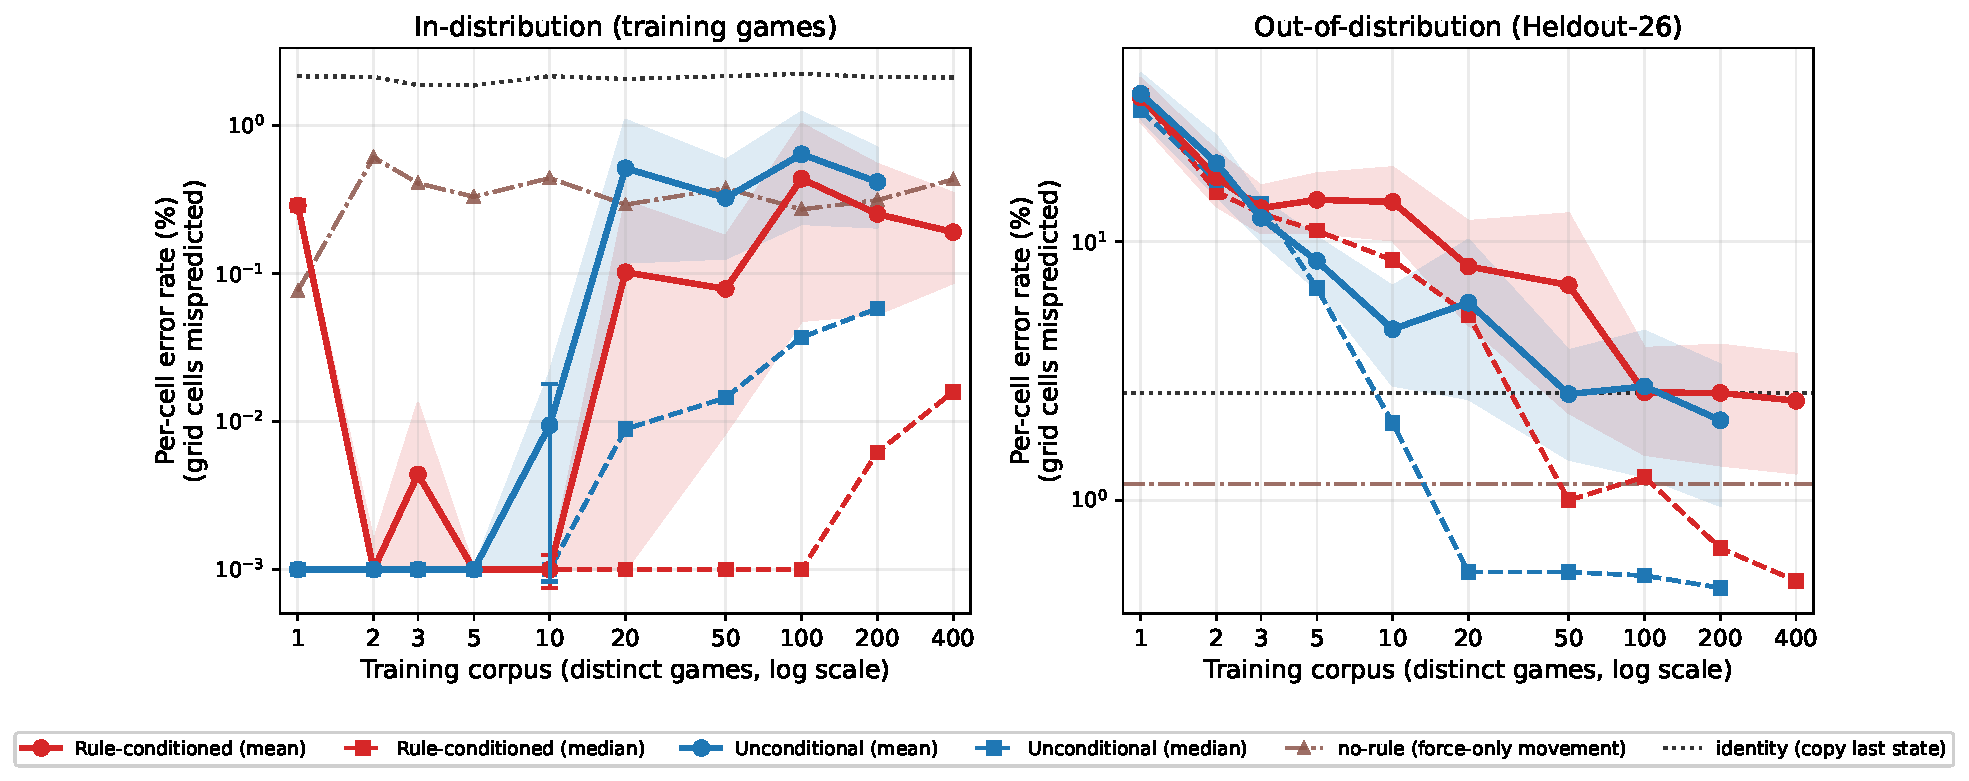
\includegraphics[width=\linewidth]{n_per_rule_slope.pdf}
\end{center}

\vspace{0.5em}
\captionsetup{labelformat=empty}
\captionof{figure}{\textbf{Data-scaling of the NCA world model vs.\ training-corpus
size.}
Each panel plots per-cell error rate (the fraction of grid cells whose
predicted object-stack differs from the ground truth, averaged over
teacher-forced rollout steps and over games) against the number of distinct
training games, selected in ascending rule-count order from the
token-deduplicated pool (the \texttt{n\_per\_rule} sweep), on log--log axes.
\emph{Left:} in-distribution, aggregated over each corpus's own training
games. \emph{Right:} out-of-distribution, aggregated over the fixed
Heldout-26 set of unseen games.
Two parameter-matched models are compared: the rule-conditioned model
($n_h{=}256$ plus the text-encoder/decoder/slot stack, ${\approx}15.97$M
parameters) and an unconditional model given slightly more capacity
($n_h{=}288$, ${\approx}16.61$M), so any conditioning benefit cannot be
attributed to parameter count.
Solid lines are the mean over games (or heldout pairs); dashed lines are the
median. The shaded band is a bootstrap 95\% confidence interval of the mean
\emph{across games} (left) or \emph{across heldout pairs} (right). The capped
vertical error bars show the \emph{across-seed} spread (min--max of the
per-seed mean), drawn only at corpus sizes with at least two training seeds;
they measure run-to-run reproducibility and are distinct from the
across-game band. The dotted black reference is the identity (copy-last-state)
baseline---per-corpus state churn in-distribution (${\approx}2\%$) and
$2.60\%$ on Heldout-26.
In-distribution error stays near zero and dilutes only mildly as the corpus
widens at fixed capacity, with the rule-conditioned mean degrading more slowly
than the unconditional one; out-of-distribution error falls toward the
identity baseline as the corpus grows.}

\end{document}
